% !TeX root = ../mythesis.tex
% !TeX encoding = UTF-8
% !TeX spellcheck = en_US

\chapter{Algorithms and Data Structures}

In this chapter we give a short overview on some basic, useful, and necessary techniques for a reasonable prover. We assume familiarity with algorithms and data structures as taught in many basic courses in computer science, e.g.\ sequences, trees, tries, etc. Still we will state some definitions and notions.
First we take a look at methods to practically achieve saturation in Section~\vref{sec:saturation:basics}.
Then we discuss some basics to speed up the retrieval of
suitable clauses and literals in Section~\vref{sec:term:indexing}.



% \section{Data structures}

% \begin{enumerate}
% 	\item Trees as first order literals, i.e.\ the root symbol is either a (negated) predicate symbol or the (negated) equality symbol.
% 	\item Multisets of literals for first order clauses
% 	\item Sets for Problems, i.e.~sets of clauses
% \end{enumerate}

% \subsection{Terms, Atoms, and Literals}

% The recursive definition of the syntax of terms, atoms and literal suggests a tree data structure.


% \begin{tikzpicture}[->,>=stealth',level/.style={sibling distance = 2cm/#1,
% 	level distance = 0.8cm}]

% \node { \( \lnot \) }
% 	child {
% 		node { \( \mP \) }
% 		child { node {\( x \)} }
% 		child { node {\( \mf \)}
% 			child { node {\( x \)} }
% 		}
% 	}
% ;
% \end{tikzpicture}

% \begin{tikzpicture}
% \draw (0,0) rectangle (1,1);
% \draw (0.1,0.1) rectangle (1cm,1cm);

% \draw (0,0) to (1,1);
% \end{tikzpicture}

% \subsection{Sets}

% Clauses are defined as multisets of literals.



\section{Practical Saturation Basics}\label{sec:saturation:basics}

In the examples of Chapter~\ref{chapter:automation},
we just applied derivation rules
to haphazardly chosen pairs of clauses
to infer new clauses
until we could conclude unsatisfiability.
%
In practice, such an approach may fail for an unsatisfiable set of clauses
simply because an important clause pairing is overlooked
and an infinite number of inferences can be drawn
from a satisfiable subset of clauses.
%
In Chapter~\ref{chapter:completeness}, on the other hand,
we relied on a fair ---
i.e.\ every non-redundant clause will be processed eventually ---
saturation process to show completeness of \InstGenEQ{}.

For now we will ignore possible simplifications of the set of clauses.
In Section~\ref{sec:given:clause:algorithm}
we will combine the given clause algorithm
and a basic selection strategy to a a simple and fair saturation process
that eventually determines all possible derivate clauses
with respect to ordered resolution.
Surprisingly the same approach will fail easily for \InstGen{}.
We consider a better suited bookkeeping of processed clauses and literals
in Section~\ref{sec:selected:literals:bookkeeping}.


% Both algorithms are just only building blocks for fair saturation strategies as we outline in Section~\ref{sec:fair:saturation:strategies:basics}

\subsection{Given Clause Algorithm}\label{sec:given:clause:algorithm}

The given clause algorithm is originated in the set of support strategy~\cite{Wos:1965:ECS:321296.321302}. (todo: Otter and discount loops~\cite{DBLP:conf/cade/SchulzM16})
%\cite{10.1007/978-3-319-40229-1_23, DBLP:conf/cade/SchulzM16})

\begin{procedure}[Given Clause Algorithm]\label{proc:given:clause:algorithm}
	We start with an empty set \( P \) of \coloremph{processed} clauses \( P \)
	and the original set of \coloremph{unprocessed} clauses \( U = S \),
	e.g.\ a set of axioms and a negated conjecture.
	\begin{enumerate}
		\item[\jek]
		If we can conclude unsatisfiability of the original set \( S \)
		then we exit the procedure with \( \UNSAT[(S)] \).
		This depends on the used calculus.
		\setcounter{enumi}{0}
		\item If there are no unprocessed clauses,
		we exit the procedure and return \(\SAT[(S)]\).
		\item We select the \coloremph{best} unprocessed clause --- the now given clause \( \mcG \) --- and remove it from the unprocessed clauses. \jek{}
		\item We check for applicable inference rules for pairs
		of the given clause with processed clauses.
		We add derived clauses to the unprocessed clauses. \hfill\jek{}
		\item We add the given clause to the processed clauses.
		We continue with step 1.
	\end{enumerate}
\end{procedure}

% \subsubsection{Ordered Resolution}

\begin{remark}
	\((\text{\Lightning}) \Leftarrow (\emptyclause\in S_i) \).
With \emph{Resolution} we conclude unsatisfiability of \( S \) whenever the (already present or derived) empty clause is encountered.
New clauses are disjunctions of instances of an active and the given clause where conflicting literals were removed,
in other words the union of the two instances without the contradicting literals.
\begin{gather*}
\infer[\sigma=\{ x'\mapsto\mf(x), y\mapsto\mg(y') \}]{
	(\mcC \lor \mcD)\sigma
}{
	\mP(\mf(x), y) \lor \mcC & \lnot\mP(x',\mg(y')) \lor \mcD
}
\end{gather*}
\end{remark}

A crucial part is the selection of the \emph{best} unprocessed clause.
At least we have to ensure that any (non-redundant) clause is selected eventually.
Otherwise we may stay in a satisfiable subset of the set of clauses
as we demonstrate in the following silly example\footnote{
In the examples the given clause is boxed,
the processed clauses are left of the given clause,
and the unprocessed clauses are right of the given clause.
Each line represents one iteration of the procedure.
}
with respect to resolution.

\begin{example}[Insufficient clause selection]
	We process the clearly unsatisfiable set of clauses
	\( S = \{
		\msucc(x)\mNE \msucc(y)\lor {x\mEQ y},
		\msucc(x_2)\mNE x_2, \msucc(x')\mEQ x'
		\} \)
	and always select the \coloremph{newest} unprocessed clause as the \emph{best} clause
	after we have moved the first clause to the processed clauses.

	\begin{align*}
		(k=1)\quad
		&\boxed{\msucc(x)\mNE \msucc(y)\lor {x\mEQ y}} &
		&&
		&{ \msucc^1(x_2)\mNE \msucc^0(x_2) },\ { \msucc(x')\mEQ x' }
		\\
		(k=2)\quad
		&\msucc(x)\mNE \msucc(y)\lor \underline{x\mEQ y} &
		&&
		&\boxed{ \msucc^1(x_2)\mNE \msucc^0(x_2) }\ \ldots
		\\
		(k=3)\quad
		&\msucc(x)\mNE \msucc(y)\lor \underline{x\mEQ y} &
		&{\left(\msucc^{i-1}(x_{i})\mNE \msucc^{i-2}(x_{i})\right)}_{i=2}^{2} &
		&\boxed{ \msucc^2(x_3)\mNE \msucc^1(x_3) }\ \ldots
		\\
		(k=4)\quad
		&\msucc(x)\mNE \msucc(y)\lor \underline{x\mEQ y} &
		&{\left(\msucc^{i-1}(x_{i})\mNE \msucc^{i-2}(x_{i})\right)}_{i=2}^{3} &
		&\boxed{ \msucc^3(x_4)\mNE \msucc^2(x_4) }\ \ldots
		\\
		\cdots\quad & \cdots && \cdots && \cdots
		\\
		(k>3)\quad
		&\msucc(x)\mNE \msucc(y)\lor \underline{x\mEQ y} &
		&{\left(\msucc^{i-1}(x_{i})\mNE \msucc^{i-2}(x_{i})\right)}_{i=2}^{k-1} &
		&\boxed{ \msucc^{k-1}(x_{k})\mNE \msucc^{k-2}(x_{k}) }
		\end{align*}
		In each iteration the newest clause
		(an instance of the second clause)
		clashes with the first clause but no other of the so far processed clauses.
		\begin{gather*}
			\infer[
				\{x\mapsto\msucc^{k-1}(x_{k}),
				y\mapsto\msucc^{k-2}(x_{k})\}
				]{
					\begin{array}{c}
					\msucc(\msucc^{k-1}(x_{k}))\mNE \msucc(\msucc^{k-2}(x_{k}))
					\\ \equiv \\
					\msucc^{k}(x_{k+1})\mNE \msucc^{k-1}(x_{k+1})
					\end{array}
				}{
				\msucc(x)\mNE \msucc(y)\lor \underline{x\mEQ y} &
				\msucc^{k-1}(x_{k})\mNE \msucc^{k-2}(x_{k+1})
			}
		\end{gather*}
\end{example}



\begin{definition}[First-in/First-out clause selection~\cite{DBLP:conf/cade/SchulzM16, DBLP:conf/cade/2016}]
	We keep track of the order clauses were added (e.g.\ by a queue).
	We restrict selection and adding of clauses
	in Procedure~\ref{proc:given:clause:algorithm} as follows:
	\begin{enumerate}
		\item[2.]
		We select the \coloremph{oldest} unprocessed clause as the \emph{best} or given clause.
		\item[3.]
		We add any derived clause
		as so far \emph{youngest} unprocessed clause.
	\end{enumerate}
	Apparently we will not miss any clause pairing.
\end{definition}



\begin{example}
	We start with the clearly unsatisfiable set of clauses
\( S=\{ \, \mP(\ma)\lor\mQ(\ma), \mP(\ma)\lor\lnot\mQ(y), \lnot\mP(x) \, \} \).
	We assume \( \mP(\ma)\succ\mQ(\ma) \),
	we underline the maximal literal in the given clauses,
	we tint conflicts red,
	 and we derive the empty clause in the fifth iteration.

	\begin{align*}
	^{1:}&\boxed{\underline{\mP(\ma)}\lor\mQ(a)}
	& ^{2:}&\mP(\ma)\lor\lnot\mQ(y) & ^{3:}&\lnot\mP(x)
	\\
	^{1:}&\mP(\ma)\lor\mQ(a)
	& ^{2:}&\boxed{\underline{\mP(\ma)}\lor\lnot\mQ(y)} & ^{3:}&\lnot\mP(x)
	\\
	^{1:}&{\colLo\mP(\ma)}\lor\mQ(a)
	& ^{2:}&{\colLo\mP(\ma)}\lor\lnot\mQ(y)
	& ^{3:}&\boxed{\underline{\lnot\mP(x)}}
	& ^{1,3:}&\mQ(\ma)
	& ^{2,3:}&\lnot\mQ(y)
	\\
	^{1:}&\mP(\ma)\lor\mQ(a)
	& ^{2:}&\mP(\ma)\lor{\colLo\lnot\mQ(y)}
	& ^{3:}&\lnot\mP(x)
	& ^{1,3:}&\boxed{\underline{\mQ(\ma)}}
	& ^{2,3:}&\lnot\mQ(y)
	& ^{2,(1,3):}&\mP(\ma)
	\\
	^{1:}&\mP(\ma)\lor{\colLo\mQ(a)}
	& ^{2:}&\mP(\ma)\lor\lnot\mQ(y)
	& ^{3:}&\lnot\mP(x)
	& ^{1,3:}&\colLo\mQ(\ma)
	& ^{2,3:}&\boxed{\underline{\lnot\mQ(y)}}
	% ^{2,(1,3):}_{1,(2,3):}\mP(\ma)
	& ^{(1,3),(2,3):}&\emptyclause
	\end{align*}
\end{example}

% \subsubsection{InstGen}

\begin{remark}
\( \text{(\Lightning)} \Leftarrow \UNSAT(S_i\bot) \).
With \InstGen{} we conclude unsatisfiability of \( S \) whenever (a subset of) \( S_i\bot \) --- a set of ground instances --- is unsatisfiable.
We consider only proper instances of a processed or given clause
as probable new clauses to extend the set of unprocessed clauses.
\end{remark}
\vspace{-1em}
\begin{gather*}
	\infer[\sigma=\{ x'\mapsto\mf(x), y\mapsto\mg(y') \}]{
		\mP(\mf(x),\mg(y')) \lor\mcC\sigma
		\qquad
		\lnot\mP(\mf(x),\mg(y'))\lor\mcD\sigma
	}{
		\mP(\mf(x), y) \lor \mcC & \lnot\mP(x',\mg(y')) \lor \mcD
	}
\end{gather*}

The following example demonstrates that the basic given clause algorithm is not suitable for \InstGen.

\begin{example}
	Again we start with the clearly unsatisfiable set of clauses
\( S=\{ \, \mP(\ma)\lor\mQ(\ma), \mP(\ma)\lor\lnot\mQ(y), \lnot\mP(x) \, \} \).
	The processed and given clauses are already encoded and
	given to a \SAT{} or \SMT{} solver.
	The basic given clause algorithm would stop and fail after \( (4) \)
	since \( S_4\bot \) is still satisfiable and there is no conflict between the underlined selected literal of the given clause
	and any selected literals of any of the processed clauses.

	\begin{align*}
	(1)\quad^{1:}&\boxed{\underline{\mP(\ma)}\lor\mQ(\ma)}
	& ^{2:}&\mP(\ma)\lor\lnot\mQ(\consbot/y)
	& ^{3:}&\lnot\mP(\consbot/x)
	\\
	(2)\quad^{1:}&{\colHi\underline{\mP(\ma)}}\lor\mQ(\ma)
	& ^{2:}&\boxed{\underline{\mP(\ma)}\lor\lnot\mQ(\consbot/y)}
	& ^{3:}&\lnot\mP(\consbot/x)
	\\
	(3)\quad^{1:}&{\colHi\underline{\mP(\ma)}}\lor\mQ(\ma)
	& ^{2:}&{\colHi\underline{\mP(\ma)}}\lor\lnot\mQ(\consbot/y)
	& ^{3:}&\boxed{\underline{\lnot\mP(\consbot/x)}}
	& ^{1,3:}_{2,3:}&\lnot\mP(\ma)
	\\
	(4)\quad
	^{1:}&{\colLo\mP(\ma)}\lor\colHi\mQ(\ma)
	& ^{2:}&{\colLo\mP(\ma)}\lor\colHi\lnot\mQ(\consbot/y)
	& ^{3:}&{\colHi\underline{\lnot\mP(\consbot/x)}}
	& ^{1,3:}_{2,3:}&\boxed{\underline{\lnot\mP(\ma)}}
	\end{align*}
	But the model did change in (4) and the selected literals of two of the processed clauses had to be changed too.
	Already processed clauses with changed selected literals have to be moved back to the unprocessed clauses.
	Then we hit a contradiction of ground instances in (7').
	\begin{align*}
	(4')\quad^{3:}&{\underline{\colHi\lnot\mP(\consbot/x)}}
	& ^{1,3:}_{2,3:}&\boxed{\underline{\lnot\mP(\ma)}}
	& ^{1:}&{\colLo\mP(\ma)}\lor\colHi\mQ(\ma)
	& ^{2:}&{\colLo\mP(\ma)}\lor\colHi\lnot\mQ(\consbot/y)
	\\
	(5')\quad^{3:}&{\underline{\colHi\lnot\mP(\consbot/x)}}
	& ^{1,3:}_{2,3:}&\colHi\underline{\lnot\mP(\ma)}
	& ^{1:}&\boxed{{\colLo\mP(\ma)}\lor\colHi\underline{\mQ(\ma)}}
	& ^{2:}&{\colLo\mP(\ma)}\lor\colHi\lnot\mQ(\consbot/y)
	\\
	(6')\quad^{3:}&{\colHi\underline{\lnot\mP(\consbot/x)}}
	& ^{1,3:}_{2,3:}&\colHi\underline{\lnot\mP(\ma)}
	& ^{1:}&{\colLo\mP(\ma)}\lor\colHi\underline{\mQ(\ma)}
	& ^{2:}&\boxed{{\colLo\mP(\ma)}\lor\colHi\underline{\lnot\mQ(\consbot/y)}}
	& ^{2,1:}&\mP(\ma)\lor\lnot\mQ(\ma)
	\\
	(7')\quad^{3:}&{\lnot\mP(\consbot/x)}
	& ^{1,3:}_{2,3:}&\colHi\lnot\mP(\tikzmark{NP}\ma)
	& ^{1:}&{\colLo\mP(\tikzmark{PP}\ma)}\lor\colN\mQ(\tikzmark{PQ}\ma)
	& ^{2:}&{\mP(\ma)\lor\lnot\mQ(\consbot/y)}
	& ^{2,1:}&\boxed{{\colLo\mP(\tikzmark{PA}\ma)}\lor\colN\lnot\mQ(\tikzmark{NQ}\ma)}
	\end{align*}

	\begin{tikzpicture}[overlay,remember picture, out=340, in=200 ]
	\draw[->, thick, dotted] (NP.south) to (PP.south);
	\draw[->, thick, dotted] (NP.south) to (PA.south);
	\draw[<->,colLo, thick] (PQ.south) to (NQ.south);
	\end{tikzpicture}
\end{example}

\subsection{Bookkeeping}\label{sec:selected:literals:bookkeeping}

Just moving processed clauses back to unprocessed clauses
as in Figure~\vref{fig:inst:gen:proving:loop}
may introduce unnecessary derivations from already considered literals.
Since we have no control over the constructed models
the selected literal of a processed clause
could be deselected in a one iteration
and re-selected in a later iteration.
Then some of the derivations of this literal against
(changed) selected literals of the processed clauses
may have already been considered
before it was deselected,
but our procedure did not keep track of that.

\begin{figure}[hbt]
	\begin{center}
		\begin{tikzpicture}[scale=0.95, transform shape]
		\node[rectangle] (start) at (0,-4em) {};
		\node (nc) [myrect] at (0,0) {new\\clauses};
		\node (pc) [myrect] at (0,8em) {unprocessed\\clauses};
		\node (ab) [myrect] at (-8em,3.5em) {instantiation};
		\node (gs) [myrect] at (-8em,8em) { \SAT};

		\node (un) [mycircle] at (-15em,8em) {
			% cspell:disable
			un\-satis\-fiable
			% cspell:enable
			};
		\node (se) [myrect] at (-8em,12.5em) {selection};
		\node (gc) [myrect] at (0em,16em) {given\\clause};
		\node (ac) [myrect,dashed] at (-13em,16.5em) {processed\\clauses};

		\node (sl) [myrect, thick] at (8.5em,12.5em) {selected literal};
		\node (us) [myrect,very thick,
		%		minimum width=8em, minimum height=3.5em, text width=7em
		] at (8.5em,8em) { \InstGen};
		\node (sa) [mycircle] at (16em,8em) {
			% cspell:disable
			satis\-fiable
			% cspell:enable
			};
		\node (su) [myrect] at (8.5em,3.5em) {substitution};

		\draw[myarrow] (start) to (nc);
		\draw[myarrow] (nc) to (pc);
		\draw[myarrow] (nc.west)  to [bend left=10] (ab);
		\draw[myarrow] (ab) to (gs);
		\draw[myarrow] (gs) to (un);
		\draw[myarrow] (gs) to (se);
		\draw[myarrow] (pc) to (gc);
		\draw[myarrow] (se.north) to [bend left=10] (gc.west);
		\draw[myarrow] (us) to (sa);
		\draw[myarrow] (us) to (su);
		\draw[myarrow] (su) to [bend left=10] (nc.east);
		\draw[myarrow] (sl) to (us);
		\draw[myarrow] (gc.east) to [bend left=10] (sl.north);
		\draw[myarrow,dashed] (gc.north) to [bend right=15](ac);

		\draw[myarrow,dotted] (ac.east) to [bend left=25](pc);

		\end{tikzpicture}
		\caption{Proving loop with \SAT{} and \InstGen{}}\label{fig:inst-gen-maxcomp}\label{fig:inst:gen:proving:loop}
	\end{center}
\end{figure}

\subsubsection{Inst-Gen}

With \InstGen{} we should keep track of already considered pairs of literals (of clauses) as we demonstrate in the following example.

\begin{example}[InstGen]
	The first two clauses have been processed before step \( m \).
	The first clause moves to the unprocessed clauses in step \( m \)
	and could have been processed again before step \( n \).
	The first clause moves again to the unprocessed clauses in step \( n \).
When the first clause is processed after step \(n \)
its selected literal clashes again with the selected literal of
the second clause.
\begin{align*}
	^{1:}&\underline{\mP(x)}\lor L_1
	&^{2:}&\underline{\lnot\mP(\ma)}\lor L_2
	&&\textcolor{colG}{\cdots}
	&\textcolor{colG}{^{i:}}&\textcolor{colG}{L_1\lor L_2}
	&\textcolor{colG}{^{j:}}&\textcolor{colG}{\lnot L_1\lor\lnot L_2}
	&&\textcolor{colG}{\cdots}
	&\textcolor{colG}{^{1,2:}}&\textcolor{colG}{\mP(\ma)\lor L_1}
	\\
	(m)\quad
	^{1:}&\mP(x)\lor \underline{L_1}
	&^{2:}&\underline{\lnot\mP(\ma)}\lor L_2
	&&\cdots
	&^{i:}&\boxed{\underline{L_1}\lor L_2}
	&\textcolor{colG}{^{j:}}&\textcolor{colG}{\lnot L_1\lor\lnot L_2}
	&&\textcolor{colG}{\cdots}
	&&\textcolor{colG}{\cdots}
	\\
	&\vdots
	\\
	(n)\quad
	^{1:}&\underline{\mP(x)}\lor {L_1} &
	^{2:}&\underline{\lnot\mP(\ma)}\lor L_2 &
	&\cdots&
	^{i:}&{L_1}\lor \underline{L_2} &
	^{j:}&\boxed{\underline{\lnot L_1}\lor \lnot L_2} &
	&\textcolor{colG}{\cdots}
\end{align*}
\end{example}

\noindent
So we maintain suitable data structure to adapt to the changed circumstances.

\begin{procedure}[Given clause algorithm for \InstGen]
	We keep track of processed pairings of clauses
	 with their (at the time of processing) selected literals
	 \( \{ (\mcC, \sel(\mcC), (\mcD,\sel(\mcD))) \} \)
	 in a suitable data structure.
	In general we proceed as in Procedure~\vref{proc:given:clause:algorithm}
	with two modifications.

	\begin{enumerate}
		\item[2.]
		After we have selected the \emph{best} unprocessed clause \( \mcG \)
		we update our model. We move processed clauses back to unprocessed
		if their selected literals have changed with the updated model.
		\item[3.]
		We only consider a processed clause with its selected literal \( (\mcC, \sel(\mcC)) \)
		if the pairing \( \{ (\mcC, \sel(\mcC)), (\mcG, \sel(\mcG)) \} \)
		is not yet recorded.
		After we have added all possible conclusions
		to the unprocessed clauses we record
		the pairing \( \{ (\mcC, \sel(\mcC)), (\mcG, \sel(\mcG)) \} \).

	\end{enumerate}



\end{procedure}

\subsubsection{Inst-Gen-Eq}

Unfortunately just keeping track of literal pairs is not enough since we construct proof trees for the contradiction from multiple literals.
Additionally we have to instantiate all clauses that contributed literals
to the proof tree with proper instantiators that were constructed along the steps of the proof.
More sophisticated approaches that addresses both problems at once are discussed in detail in~\cite{CS2011PhD}.




% \begin{align*}
% 	\textcolor{colHi}{\mP}\lor\mQ\lor\mR
% 	\\
% 	\mP\lor\textcolor{colHi}{\mQ}\lor\mR
% 	&&\lnot\mP\lor \textcolor{colHi}{\mQ} \lor \mR
% 	\\
% 	\mP\lor\textcolor{colHi}{\mQ}\lor\mR
% 	&&\lnot\mP\lor \textcolor{colHi}{\mQ} \lor \mR
% 	&&\mP\lor\lnot\mQ
% \end{align*}





% \subsection{An insufficient strategy}







\section{Term Indexing}\label{sec:term:indexing}





%“Implementations of theorem provers that use generative procedures like resolution (Robinson, 1965b; Chang and Lee, 1973) or Knuth-Bendix completion (Knuth and Bendix, 1970) face the problem of program degradation: The theorem prover`s rate of drawing conclusions falls off sharply with time due to an increasing amount of retained information (Wos, 1992). \cite{Graf1998}



A refutation theorem proving process like \InstGenEQ{} produces a lot of clauses.
For each occurring clause, we have to find
all other clauses that match specific conditions to preserve completeness.
First of all, of course, we want to avoid unnecessary clauses in our set of processed clauses
--- at least we might expect that we do not have to process multiple variants of a clause.
Further we search for processed clauses that contain clashing literals to our selected literal in our given clause.
In the presence of equality we search for subterms in selected literals of processed clauses that unifies with one side of the selected equation in our given clause.

Naively we can just scan through all existing clauses (selected literals)
and check each clause (selected literal) for the desired properties.
	Then the workload for processing one additional clause is proportional to the number of other clauses and
	the workload for checking a pair of clauses.
	The latter includes unification, which is at least linear to the size of clauses~\cite{ALBERT19933},
	while Robinson's unification algorithm~\cite{Robinson:1965:MLB:321250.321253} is exponential in the worst case.
	The complexity class for this direct approach of processing \( n \) clauses of a maximal size
	(i.e.\ constant bound for unification costs per pair) is \( \mcO(n^2) \).

	Term indexing~\cite{Graf1998} is about data structures and algorithms
	for faster retrieval of matching clauses, literals, and terms.
	We will introduce the used notions for term indexing, describe
	use cases, data structures, and algorithms for the indexing
	of clauses, literals, and terms and the corresponding algorithms
	for fast retrievals of sets of candidate clauses that likely matches the desired properties.

	\begin{remark}
		The following Definitions~\ref{def:position:string} to~\ref{def:agnostic:position:string}
		are easily applicable to functional and literal terms, but not to clauses (i.e.\ sets of literals).
		Primarily we will build indexes over from literal terms.
	\end{remark}

	\begin{definition}\label{def:position:string}
		A \coloremph{position string} \( \ANGLES{p, s } \)
		is a pair of a position \( p \) and a symbol \( s \),
		i.e.~negation, predicate, equation, function, constant, variable.
%
		We define the set of position strings \(\PosStr(t)\)
		of a term \( t \) as follows.
		\begin{gather*}
		\PosStr(t) =
		\begin{cases}
		\{ \ANGLES{\epsilon,x} \}
		& \text{if }t=x\in\SIGV \\
		\{ \ANGLES{\epsilon, \mcf} \} \cup \{ \ANGLES{ip,s}\mid \ANGLES{p,s} \in\PosStr(t_i)\}
		&\text{if }t=\mcf(t_1,\ldots,t_n)
		\end{cases}
		\end{gather*}
	\end{definition}



	\begin{definition}\label{def:term:path}
		A \coloremph{term path} in a term \( t \)
		is a finite sequence
		\( {( \ANGLES{p_i,s_i} )}^{n}_{i=1}
			\)
		of position strings such that
		\( \ANGLES{p_i,s_i} \in \PosStr(t) \),
		and \( p_i = p_{i-1} k_i \)
		for all \( i > 1 \)
		and some \( k_i \in\mathbb{N} \),
		i.e.~\(p_{i-1}\) is the longest proper prefix of \(p_{i}\).


	\end{definition}

	\begin{definition}\label{def:term:traversal}
		A \coloremph{term traversal} of a term \( t \)
		is a finite sequence
		\( {( \ANGLES{p_i,s_i} )}^{n}_{i=1}
			\)
		of position strings such that
		\( n = |\PosStr(t)| \) and
		\( \bigcup_{i=1}^{n} \{\ANGLES{p_i,s_i}\} = \PosStr(t) \),
		i.e.~\( p_i \neq p_j \) for all \( i \neq j\).

		% \begin{gather*}
		% \MDEFINE[:\Leftrightarrow]{p \prec q}{clc}{
		% 	p < q & p\text{ is a proper prefix of }q
		% 	\\
		% 	i < j & \text{if }p=ras, q=rbt, a\in\mathbb{N}, b\in\mathbb{N}
		% }
		% \end{gather*}

		A pre-order term traversal
		\( {( \ANGLES{p_i,s_i} )}^{n}_{i=1} \)
		is a term traversal such that whenever \( i < j \)
		% for \( \ANGLES{p_i,s_i} \) and \( \ANGLES{p_j,s_j} \)
		then either position
		\( p_i \) is \emph{above} position \( p_j \)
		or position \( p_i \) is \emph{left} of position \( p_j \)
		(see Definition~\vref{def:position} for above and left).
	\end{definition}
%
	\begin{example}
		We express term paths and term traversals
		with position strings,
		e.g.\ for literal term \( \mP(\mf(\ma, y )) \) we have \( \PosStr(
			{\mP(\mf(\ma, y ))}
			) = \{
			\ANGLES{\epsilon,\mP},
		\ANGLES{1,\mf},
		\ANGLES{11,\ma},
		\ANGLES{12,y}
		\}
		\).
		\\[-0.5em]
	\begin{minipage}[c]{10.5cm}
		\begin{gather*}
			% {\ANGLES{\epsilon,\mh}\ANGLES{1,\mf}\ANGLES{11,\ma}
			% \tag*{{path from root to leaf \( \ma \) (---)}}
			% }
			% \\
			{\ANGLES{\epsilon,\mP}\ANGLES{1,\mf}\ANGLES{12,y}
			\tag*{{path from root to leaf \( y \) (dashed)}}
			}
			\\
			{\ANGLES{\epsilon,\mP}\ANGLES{1,\mf}\ANGLES{11,\ma}\ANGLES{12,y}
			\tag*{{pre-order traversal (dotted)}}
			}
		\end{gather*}
		Root position \( \epsilon \) is a above positions \(1, 11, 12\);
		position \( 1 \) is above positions \(11, 12\);
		position \( 11 \) is left of position \( 12 \).
	\end{minipage}
	\qquad
	\begin{minipage}[c]{4.1cm}
		\begin{tikzpicture}[right]
		{\node (h) at (0,-1) {\( \ANGLES{\epsilon,\mP} \)};}
		{\node (hf) at (0,-2) {\( \ANGLES{1,\mf} \)};}
		{\node (hfa) at (-1,-3) {\( \ANGLES{11,\ma} \)};}
		{\node (hfy) at (1,-3) {\( \ANGLES{12,y} \)};}
		% \node (x) at (0,-0.5) {.};
		%
		{\path[->,dashed]
			(h) edge (hf)
			(hf)
			edge (hfy)
			;}
		{\path[->,dotted, bend right]
			(h) edge (hf)
			(hf) edge (hfa)
			(hfa) edge[bend left] (hfy)
			;}
		\end{tikzpicture}
	\end{minipage}
\end{example}

\begin{notation}\label{notation:term:path}
	Since \( p_{i} = p_{-1} k_{i} \) for
	all \( i > 1 \) and
	some \( k_{i+1}\in\mathbb{N} \)
	we abbreviate term paths by omitting the prefixes in positions strings
	\( \ANGLES{p_{i-1} k_{i}, s_{i}} \) for \( i>1 \) without ambiguity.
	\[
		{(\ANGLES{p_i, s_i })}_{i=1}^n
		=
		\ANGLES{p_1,s_1}{(\ANGLES{p_{i-1}k_i, s_i })}_{i=2}^n
		\simeq
		\ANGLES{p_1,s_1}
		{(\ANGLES{k_i, s_i })}_{i=2}^n
		\simeq
		p_1.s_1{(.k_i.s_i)}_{i=2}^n
	\]
	Additional we omit angles. For readability we separate
	positions and symbols with dots.
	\begin{gather*}
		\ANGLES{11,\mf} \ANGLES{112,y}
		\simeq
		\ANGLES{11,\mf} \ANGLES{2,y}
		\simeq
		11.\mf.2.y
		\\
		\ANGLES{\epsilon,\mP} \ANGLES{p1,\mf} \ANGLES{p12,y}
		\simeq
		\ANGLES{\epsilon,\mP} \ANGLES{1,\mf} \ANGLES{2,y}
		\simeq
		\mP.1.\mf.2.y
	\end{gather*}
\end{notation}

\begin{notation}\label{notation:term:traversal}
	Since the arities of symbols are fixed
	and the pre-order term traversal is unique for any term
	we omit angles and positions.
	For readability we separate symbols with dots.
	\[
		\ANGLES{\epsilon,\mP} \ANGLES{1,\mf} \ANGLES{11,\ma} \ANGLES{12,y}
		\simeq
		\mP.\mf.\ma. y
	\]
\end{notation}

\begin{definition}[Normalization]\label{def:variable:normalization}
% A variable \(x\) occurs prior to variable \(y\) in term \( t \)
% if there exists a position \(p\) with \( \ANGLES{p,x} \in \PosStr(t) \)
% such that position \(p\) is left of any position \(q\)
% where \( \ANGLES{q,y} \in \PosStr(t) \).
%
A term \( t \) is normalized
with respect to a sequence of variables \( {(x_i)}_{i=1}^\infty \)
if \( \var(t) = \bigcup_{i=1}^n\{ x_i \} \) for some \( n \in \mathbb{N} \)
and for any \( i < j \leq n \) the variable
\( x_i \) occurs \emph{left} (see Definition~\vref{def:position})
of variable \( x_j \) in term \( t \).
A substitution \( \sigma \) \coloremph{normalizes} term \( s \)
with respect to \( {(x_i)}_{i=1}^\infty \)
iff \( \sigma \) is a variable renaming and
\( s\sigma \) is normalized with respect to \( {(x_i)}_{i=1}^\infty \).

\end{definition}

\begin{definition}\label{def:agnostic:position:string}
	We define the set of variable agnostic position strings \(\vaPosStr(t)\)
		of a term \( t \) with fresh symbol \( * \) as follows.
		\begin{gather*}
		\vaPosStr(t) =
		\begin{cases}
		\{ \ANGLES{\epsilon,*} \}
		& \text{if }t=x\in\SIGV
		\\
		\{ \ANGLES{\epsilon, \mcf} \} \cup \{ \ANGLES{ip,s}\mid \ANGLES{p,s}
		\in\vaPosStr(t_i)\}
		&\text{if }t=\mcf(t_1,\ldots,t_n)
		\end{cases}
		\end{gather*}
\end{definition}

\begin{example}
	Term paths and term traversals work properly with
	variable agnostic positions strings.
	\begin{align*}
		\mP(\mf(x,y),z)
		&\Rightarrow
		\mP.1.\mf.1.*, \mg.1.\mf.2.*, \mg.2.*
		\tag*{term paths from root to leafs}
		\\
		&\Rightarrow \mP.\mf.*.*.*
		\tag*{pre-order traversal}
	\end{align*}
\end{example}

\subsection{Use cases}

We now look at some applications of term indexing in the context of 
\InstGen{} and \InstGenEQ{}.

\subsubsection{Clashing literals}

For theorem proving with \InstGen 
we have to search quickly for clashing selected literals.

% PATH INDEXING/PrefixTrees
\begin{example}
	We have constructed the variable agnostic literals tree
	for the following literals:
	\begin{gather*}
	\{
	\TI{1}\mP(\mf(x,x)),
	\TI{2}\mP(\mg(\ma,x)),
	\TI{3}\mP(\mf(y,z))
	\TI{4}\mP(\mg(\ma,y)),
	\TI{5}\mP(\mf(y,x)),
	\TI{6}\mP(\mg(y,a))
	\}
	\end{gather*}
	%
	\begin{center}
		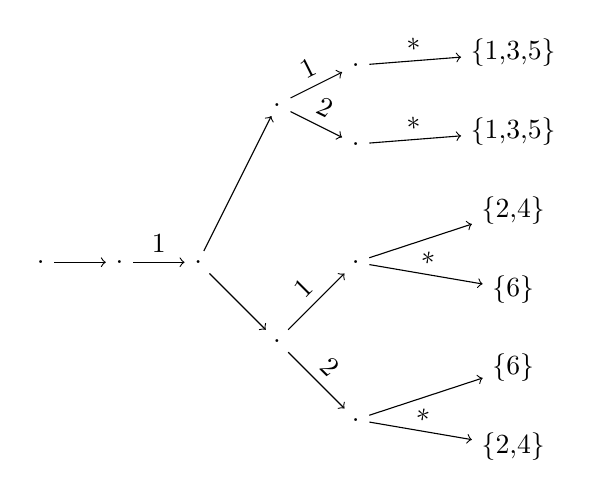
\begin{tikzpicture}[->,sloped,above]

		\node (root) at (0,2.5) {.};

		\node (h) at (1,2.5) {.};

		\node (h1) at (2,2.5) {.};

		\node (h1f) at (3,4.5) {.};
		\node (h1g) at (3,1.5) {.};

		\node (h1f1) at (4,5) {.};
		\node (h1f2) at (4,4) {.};
		\node (h1g1) at (4,2.5) {.};
		\node (h1g2) at (4,0.5) {.};

		\node (h1f1x) at (6,5) {\{1,3,5\}};
		\node (h1f2x) at (6,4) {\{1,3,5\}};
		\node (h1g1a) at (6,3) {\{2,4\}};
		\node (h1g1x) at (6,2) {\{6\}};
		\node (h1g2a) at (6,1) {\{6\}};
		\node (h1g2x) at (6,0) {\{2,4\}};

		\path
		(root) edge node {\( \mP \)} (h)

		(h) edge node {\( 1 \)} (h1)

		(h1)
		edge node {\( \mf \)} (h1f)
		edge node {\( \mg \)} (h1g)

		(h1f)
		edge node {\( 1 \)} (h1f1)
		edge node {\( 2 \)} (h1f2)

		(h1g)
		edge node {\( 1 \)} (h1g1)
		edge node {\( 2 \)} (h1g2)

		(h1f1)
		% edge node {\( \ma \)} (h1f1a)
		edge node {\( * \)} (h1f1x)

		(h1f2)
		%		edge node {\( \ma \)} (h1f2a)
		edge node {\( * \)} (h1f2x)


		(h1g1)
		edge node {\( \ma \)} (h1g1a)
		edge node {\( * \)} (h1g1x)

		(h1g2)
		edge node {\( \ma \)} (h1g2a)
		edge node {\( * \)} (h1g2x)

		;
		\end{tikzpicture}
	\end{center}
	%
	Now we retrieve candidate clauses with literals that clash with
	literal \( \lnot\mP(\mg(y',\mf(x'))) \):
%
\begin{gather*}
	\texttt{clashing}: \lnot\mP(\mg(y',\mf(x')))
	\mapsto \texttt{unifiable}: \{ \mP.1.\mg.1.{*}, \mP.1.\mg.2.\mf.1.* \}
	\mapsto \{ 2, 4, 6 \} \cap \{ 2, 4 \}
\end{gather*}
	\end{example}



\subsubsection{Redundant clauses}

In Resolution-based calculi
we can ignore or omit clauses that are subsumed
by other clauses.
Weakened instances of other clauses are redundant.
%
In contrast
we must keep keep or add subsumed clauses
with \InstGen and \InstGenEQ as 
we show with the following example and lemma.
But still we can ignore or remove some redundant clause,
but the notion of redundancy is different from resolution.

\begin{example}\label{ex:not:equisat}
	The set of clauses \( S = \{ \,
	\mP(x), \lnot\mP(\mf(\ma))
	\, \} \) is clearly unsatisfiable, but
	\( S\bot \) is still satisfiable.
	We derive \( \mP(\mf(\ma)) \) which is subsumed by \( \mP(x) \),
	but can not ignore it because \( \{ \,
	\mP(\bot), \lnot\mP(\mf(\ma)), \mP(\mf(\ma))
	\, \} \) is unsatisfiable as desired.
\end{example}

\begin{lemma}
	If \( S = S' \cup \{ \mcD \} \),
	\( \mcC \in S' \), and there is a substitution \( \sigma \)
	such that \( \mcC\sigma \subseteq \mcD \)
	then
	\( S  \equisat S' \),
	but \( S\bot  \not\equisat S'\bot \).
\end{lemma}
\begin{proof}
	Obviously \( S'\cup \{ \mcD \} \entails S' \) and
	\( \mcC\sigma\entails\mcD \) by definition, hence
	\( S' \entails S'\cup \{ \mcD \} \) and
	\( S' \equiv S'\cup \{ \mcD \} \) which implies
	\( S' \equisat S' \cup \{ \mcD \} \).
%
	Although \( S'\bot\cup \{ \mcD\bot \} \entails S'\bot \)
	we have a counterexample to
	\( S'\bot \equisat S\bot \) with Example~\ref{ex:not:equisat},
	where \( C\sigma\bot \not\entails D\bot \),
	i.e.~\( \mP(\bot)\not\entails\mP(\mf(\ma)) \), but \( \mP(x)\entails\mP(\mf(\ma))  \).
\end{proof}
\begin{lemma}[Weakened variants]\label{lem:weakend:variants}
	If \( S = S' \cup \{ \mcD \} \),
	\( \mcC \in S' \), and there is a variable substitution \( \rho \)
	such that \( \mcC\rho \subseteq \mcD \)
	then
	\( S\bot\equisat S'\bot \).
\end{lemma}
\begin{proof}
	Since \( \rho \) is a variable substitution
	\( \mcC\rho\bot \entails \mcD\bot \) holds
	because \( \mcD\bot = \mcC\rho\bot \lor \mcD' \).
\end{proof}

\begin{example}
	\(
		\{ \ldots,
		\mP(x)\lor \mQ(y), \mP(z)\lor\mQ(z) \lor \mQ(\mf(z)) \}\bot
		\equisat
		\{ \ldots, \mP(x) \lor \mQ(y) \}\bot
	\)
	since \(
		(\mP(x)\lor\mQ(y)) \{x\mapsto z, y\mapsto z \}
		\subseteq
		\mP(z)\lor\mQ(z)\lor\mQ(\mf(z))
	\).
\end{example}

\begin{definition}[Backward removal]
	For a set of processed clauses \( P \)
	and a given (derived or unprocessed) clause \( \mcG \) we
	 remove clauses \( \mcD_i \) from \( P \) where
	 \( \mcG\rho_i \subseteq \mcD_i \) for some
	 variable substitution \( \rho_i \).
\end{definition}

\begin{definition}[Forward removal]
	For a set of processed clauses \( P \)
	we can omit a given (derived or unprocessed) clause \( \mcG \)
	if there exists a clause \( \mcC \in P \)
	and a variable substitution \( \rho \) such that \( \mcC\rho\subseteq \mcG \).
\end{definition}

	\begin{example}
		With variable agnostic term traversals we may encounter
		candidates for (weakened) variants that are actually not variants.
		There is no variable renaming \( \rho \) such that
		\( R(x,x,y) \rho = R(x',y',y') \) or
		\( R(x',y',y') \rho = R(x,x,y) \)
		but \( R.*.*.* \) matches perfectly.
	\end{example}

\subsubsection{Unifiable subterms}

For \InstGenEQ we have to quickly search for unifiable subterms of selected literals to apply unit superposition.

% PATH INDEXING/SubtermTrees
\begin{example} We have constructed the prefix tree for all subterms of the following literals. We annotate the references to our literals with the positions of the subterms (starting at the atom).
	\begin{gather*}
	\{
	\TI{1}\mP(\mh(\mf(x,x))),
	\TI{2}\lnot\mP(\mh(\mg(\ma,x))),
	\TI{3}\mP(\mh(\mf(y,z))),
	\\
	\TI{4}\lnot\mP(\mh(\mg(\ma,y))),
	\TI{5}\mP(\mh(\mf(y,x))),
	\TI{6}\lnot\mQ(\mh(\mg(y,a)),\ma)
	\}
	\end{gather*}
	%
	\begin{center}
		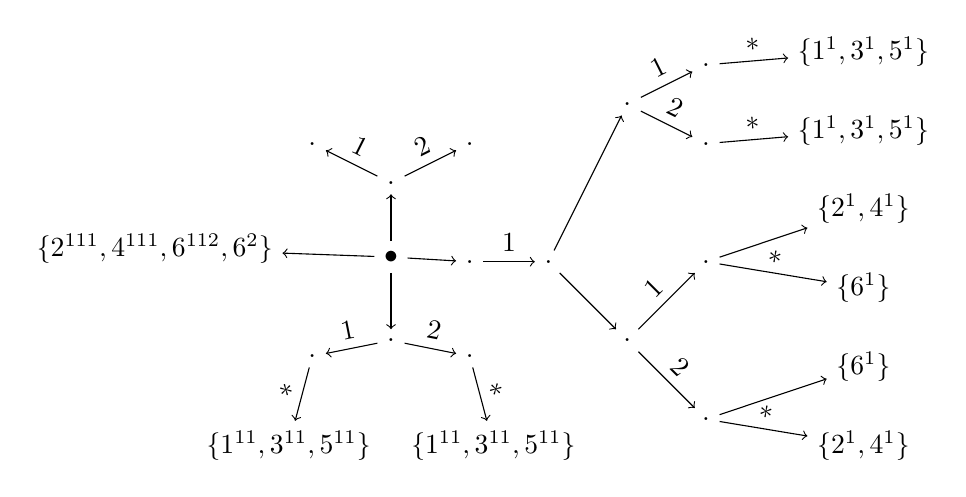
\begin{tikzpicture}[->,sloped,above]
		\node (root) at (0,2.5) {\( \bullet \)};
		%% right
		\node (h) at (1,2.5) {.};
		%
		\node (h1) at (2,2.5) {.};
		%
		\node (h1f) at (3,4.5) {.};
		\node (h1g) at (3,1.5) {.};
		%
		\node (h1f1) at (4,5) {.};
		\node (h1f2) at (4,4) {.};
		\node (h1g1) at (4,2.5) {.};
		\node (h1g2) at (4,0.5) {.};
		%
		\node (h1f1x) at (6,5) {\( \{1^1,3^1,5^1\} \)};
		\node (h1f2x) at (6,4) {\( \{1^1,3^1,5^1\} \)};
		\node (h1g1a) at (6,3) {\( \{2^1,4^1\} \)};
		\node (h1g1x) at (6,2) {\( \{6^1\} \)};
		\node (h1g2a) at (6,1) {\( \{6^1\} \)};
		\node (h1g2x) at (6,0) {\( \{2^1,4^1\} \)};
		%% down
		\node (f) at (0,1.5) {.};
		\node (f1) at (-1,1.3) {.};
		\node (f1x) at (-1.3,0) {\( \{1^{11},3^{11},5^{11}\} \)};
		\node (f2) at (1,1.3) {.};
		\node (f2x) at (1.3,0) {\( \{1^{11},3^{11},5^{11}\} \)};
		%% up
		\node (g) at (0,3.5) {.};
		\node (g1) at (-1,4) {.};
		\node (g2) at (1,4) {.};
		%% left
		\node (a) at (-3,2.5) {\( \{2^{111}, 4^{111}, 6^{112}, 6^2 \} \)};

		\path
		(root)
		edge node {\( \mh \)} (h)
		edge node {\( \mf \)} (f)
		edge node {\( \mg \)} (g)
		edge node {\( \ma \)} (a)

		(h) edge node {\( 1 \)} (h1)


		(h1)
		edge node {\( \mf \)} (h1f)
		edge node {\( \mg \)} (h1g)

		(h1f)
		edge node {\( 1 \)} (h1f1)
		edge node {\( 2 \)} (h1f2)

		(h1g)
		edge node {\( 1 \)} (h1g1)
		edge node {\( 2 \)} (h1g2)

		(h1f1)
		edge node {\( * \)} (h1f1x)

		(h1f2)
		edge node {\( * \)} (h1f2x)


		(h1g1)
		edge node {\( \ma \)} (h1g1a)
		edge node {\( * \)} (h1g1x)

		(h1g2)
		edge node {\( \ma \)} (h1g2a)
		edge node {\( * \)} (h1g2x)

		%
		(g) 	edge node {\( 1 \)} (g1)
		edge node {\( 2 \)} (g2)

		(f)	edge node {\( 1 \)} (f1)
		edge node {\( 2 \)} (f2)

		(f1)	edge node {\( * \)} (f1x)
		(f2)	edge node {\( * \)} (f2x)
		;


		\path (root)



		;

		\end{tikzpicture}
	\end{center}

	Now we retrieve literals with subterms that may be unifiable
	with terms \( \mf(\ma,\mb) \) and \( \mg(\ma,\mb) \).
	\begin{align*}
		\texttt{subterm}: \mf(\ma,\mb)
		&\mapsto \texttt{unifiable}: \{ \mf.1.\ma, \mf.2.\mb  \}
		\mapsto \{ 1^{11}, 3^{11}, 5^{11}  \}
		\\
		\texttt{subterm}: \mg(\ma,\mb)
		&\mapsto
		\texttt{unifiable}: \{ \mg.1.\ma, \mf.2.\ma  \}
		\mapsto
		\{ 2^{11}, 4^{11} \} \cap \{ 6^{11} \} = \emptyset
	\end{align*}
\end{example}
















% % !TeX root = ../mythesis.tex
% !TeX encoding = UTF-8
% !TeX spellcheck = en_US

\section{Term indexing samples}
\subsection{Motivation}
%% MOTIVATION %%

%- MOTIVATION/ClausalForm
%- MOTIVATION/Notation

%+ MOTIVATION/forwardSubsumption.tex

\begin{example}[forward subsumption]
	\begin{gather*}
	S = \{ \TI{1}\mP(x,y), \TI{2}\lnot \mP(\ma,z)\} \cup \{\TI{3}\colG\mP(\ma,z') \}
	\tag*{\( \mcC_1 \) subsumes \( \mcC_3 \)}
	\\[0.7em]
	\infer[\{x\mapsto\ma,y\mapsto z\}]
	{\square}
	{\mP(x,y) & \lnot \mP(\ma,z)}
	\tag*{Resolution}
	\\[0.7em]
	S\bot = \{ \mP(\bot,\bot), {\colLo\lnot \mP(\ma,\bot), \mP(\ma,\bot)} \}
	\tag*{InstGen / SMT}
	\end{gather*}
\end{example}

%+ MOTIVATION/goalEffectiveCalculus
%+ MOTIVATION/goalFastTermRetrieval
%+ MOTIVATION/goalSoundComplete
\begin{goal}
	%	A sound\( ^\circ \), refutational complete\( ^\diamond \), and effective\( ^\star \) calculus.
	A sound, refutation complete, and
	 {effective} calculus.
	\begin{enumerate}
		\item {Reduce} search space
		\begin{itemize}
			\item Ordered Resolution, Strategies, \ldots
			\item \ldots with selection functions for clauses and literals
		\end{itemize}
		\item {Reduce} redundancy
		\begin{itemize}
			\item e.g.~discard clauses that are subsumed by other clauses
			\item \ldots depending on the calculus
		\end{itemize}
		\item Quickly find
		\begin{itemize}
			\item {variants} \hfill{\footnotesize variant removal}

			\item {instances}   \hfill{\footnotesize backward subsumption}\\
			\( \INST(s,t)\Leftrightarrow\exists\sigma\ s = t\sigma \)

			\item {generalizations}  \hfill{\footnotesize forward subsumption}\\
			\( \GNRL(s,t)\Leftrightarrow\exists\sigma\ s\sigma = t \)

			\item {unifiable terms} \hfill{\footnotesize resolution, demodulation}\\
			\( \UNIF(s,t)\Leftrightarrow\exists\sigma\ s\sigma = t\sigma \)

		\end{itemize}

		of a query term in a given set of terms.
	\end{enumerate}
\end{goal}

\begin{definition}
	\begin{align*}
	\VRNT(s,t)&\Leftrightarrow \exists\sigma\ s\sigma = t\text{ and }\sigma\text{ is renaming}\\
	\INST(s,t)&\Leftrightarrow\exists\sigma\ s = t\sigma\tag*{\( s \) is instance of \( t \)}\\
	\GNRL(s,t)&\Leftrightarrow\exists\sigma\ s\sigma = t\tag*{\( s \) is generalization of \( t \)}\\
	\UNIF(s,t)&\Leftrightarrow\exists\sigma\ s\sigma = t\sigma
	\end{align*}
\end{definition}

\begin{tikzpicture}[scale = 1, transform shape, draw=black, fill=black, thick, sloped]

\draw[->, ultra thick] (0,0) --
node[pos=0, above] {\( F \)}
(2,0);

% outer rectangle
\draw[rounded corners=-1.5mm] (1,3) rectangle (8.5,-3);
% is F a theorem?
\draw(2.4,2.7) node {\color{colN}Is \( F \) a theorem?};

% SLIDE Is S satisfiable?
\node[colG] (S) at (1.6,-2.7) {\scriptsize\( \lnot F \approx S \)};
\node (S) at (2.5,0) {\( S \)};


% SLIDE 2
\draw[thin,dashed,draw=colO] (2.5,0) ellipse (0.4 and 1.2); % S

% inner rectangle
\draw[rounded corners=-1.5mm]  (1.5,-2.25) rectangle (8,2.25);
% is S satisfiable?
\draw (3.2,-1.9) node {\color{colN}Is \( \lnot F \) satisfiable?};

% SLIDE unsatisfiable
\draw[thin,dashed,draw=colO] (2.6,0) ellipse (0.6 and 1.44);  % S
\draw[dashed, draw=colG, thick] decorate[decoration={snake}] {(1.4, 1) -- (8.2,0.6)};
\draw[->, draw=colHi, ultra thick] (6.5,1.8) --
node[pos=0,below] {unsatisfiable}
node[pos=0.85, above] {theorem}
(10,1.8) ;

% SLIDE satisfiable
\draw[thin,dashed,draw=colO] (2.8,0) ellipse (0.9 and 1.73);  % S
\draw[dashed, draw=colG, thick]  decorate[decoration={snake}] { (1.4,-1)  --  (8.2,-0.6) };
\draw[->,draw=colLo, ultra thick] (7,-1.3) --
node[pos=0, below] {satisfiable}
node[pos=0.75, above] {not a theorem} (11,-1.3) ;

% SLIDE 5
\draw[thin,dashed,draw=colO] (3.2,0) ellipse (1.35 and 2.07); % S
\draw[->,draw=colNa, ultra thick] (7,0.15) --
%	node[pos=0,above] {space out}
node[pos=0,below] {time out}
node[pos=0.85, above] {maybe} (10.5,0.15) ;
\end{tikzpicture}

%%

\begin{definition}[Term Indexing]
	Term indexing is about data structures and algorithms for fast retrieval of matching terms.
\end{definition}


\subsection{Position}

%+ POSITION/Normalization
\begin{example}{Variable normalization}
	Variants of terms generate the same position strings
	\begin{itemize}
		\item if variable names are ignored
		\hfill \( \mf(y,z) \Rightarrow
		\ANGLES{\epsilon,\mf}
		\ANGLES{1,*}
		\ANGLES{2,*}
		 \)

		\item or normalized
		\hfill \( \mf(y,z) \Rightarrow
		\ANGLES{\epsilon,\mf}
		\ANGLES{1,x_1}
		\ANGLES{2,x_2} \)
		\\
		\hfill \( \mf(y,y) \Rightarrow
		\ANGLES{\epsilon,\mf}
		\ANGLES{1,x_1}
		\ANGLES{2,x_1}
		 \)
	\end{itemize}

	In the first case even non-variants of terms generate the same strings.
\end{example}


%+ POSITION/PositionStrings + Term traversals
\begin{definition} We define the set of \coloremph{position strings}
	\begin{gather*}
	\posS(t) =
	\begin{cases}
	\{ \ANGLES{\epsilon,x} \}
	& \text{if }t=x\in\SIGV \\
	\{ \ANGLES{\epsilon, f} \} \cup \{ \ANGLES{ip,s}\mid \ANGLES{p,s} \in\posS(t_i)\}
	&\text{if }t=f(t_1,\ldots,t_n)
	\end{cases}
	\end{gather*}
\end{definition}

\begin{example}[Term traversals]x
	%	\begin{gather*}{
	%		\PosStr(\mh(\mf(\ma,\my))) = \{
	%		{ \ANGLES{\epsilon,\mh},
	%	}}
	%	{ \ANGLES{1,\mf}, }
	%	{ \ANGLES{11,\ma}, }
	%	{ \ANGLES{12,y} }
	%	\end{gather*}

	\begin{minipage}[c]{3.1cm}
		\begin{tikzpicture}[left]
		{\node (h) at (0,-1) {\( \ANGLES{\epsilon,\mh} \)};}
		{\node (hf) at (0,-2) {\( \ANGLES{1,\mf} \)};}
		{\node (hfa) at (-1,-3) {\( \ANGLES{11,\ma} \)};}
		{\node (hfy) at (1,-3) {\( \ANGLES{12,y} \)};}
		%
		{\path[->,dashed]
			(h) edge (hf)
			(hf)
			edge (hfy)
			;}
		{\path[->,dotted, bend right]
			(h) edge (hf)
			(hf) edge (hfa)
			(hfa) edge[bend left] (hfy)
			;}
		\end{tikzpicture}
	\end{minipage}
	\begin{minipage}[c]{7.5cm}
		\begin{gather*}
		%	{
		%		\PosStr(\mh(\mf(\ma,\my))) = \{
		%		{ \ANGLES{\epsilon,\mh},
		%	}}
		%	{ \ANGLES{1,\mf}, }
		%	{ \ANGLES{11,\ma}, }
		%	{ \ANGLES{12,y} }
		%	\} \\[2em]
		{\ANGLES{\epsilon,\mh}\ANGLES{1,\mf}\ANGLES{12,y}
			\tag*{{path from root to leaf}}
			%\tag{\( \mh 1 \mf 2 y \)}
		}			\\
		{\ANGLES{\epsilon,\mh}\ANGLES{1,\mf}\ANGLES{11,\ma}\ANGLES{12,y}
			\tag*{{pre-order traversal}}
		}
		\\
		\end{gather*}
	\end{minipage}
\end{example}

%+ POSITION/Simplification
\begin{notation}
	We abbreviate
	\begin{itemize}
		\item path strings
		\( \ANGLES{\epsilon,\mh}\ANGLES{1,\mf}\ANGLES{12,*} \)
		\hfill \( \mh.1.\mf.2.{*} \)

		\item and pre-order traversal strings
		\( \ANGLES{\epsilon,\mh}\ANGLES{1,\mf}\ANGLES{11,*}\ANGLES{12,*} \)
		\hfill \( \mh.\mf.\ma.{*} \)
		\\
		when the arities of function symbols are fixed.
	\end{itemize}
\end{notation}

\subsection{Path Indexing}

%% PATH INDEXING %%

%+ PATH INDEXING/Build+Index
\begin{example}{Build}
	\def\TRIEWIDTH{4cm}
	\def\TEXTWIDTH{\textwidth-\TRIEWIDTH-2em}

	\begin{minipage}{\TEXTWIDTH}
		\(
		\TI{t_1}\,\mh(\mf(x,y)),
		\TI{t_2}\mh(\mf( x,\ma)),
		\TI{t_3}\mh(\mf(\ma,\ma))
		 \)
		\begin{align*}
		t_1 &\Rightarrow \{ \mh.1.\mf.1.{*},  \mh.1.\mf.2.{*} \} \\
		t_2 &\Rightarrow \{ \mh.1.\mf.1.{*},  \mh.1.\mf.2.\ma \} \\
		t_3 &\Rightarrow \{ \mh.1.\mf.1.\ma,  \mh.1.\mf.2 \ma \}
		\end{align*}
	\end{minipage}
%
	\begin{minipage}{\TRIEWIDTH}
	\begin{tikzpicture}[->,dotted]
%		\renewcommand{\PAUSE}{\pause}
%		\input{PATHINDEXING/Index}
\input{samples/pathindexingindex}

		\end{tikzpicture}
	\end{minipage}
\end{example}


%+ PATH INDEXING/PathStrings
\begin{example}{Path strings}
	The path-strings of \( \mh(\mf(\ma,y)) \) are
	{\( \mh. 1. \mf. 1. \ma \)} and
	{\( \mh. 1. \mf. 2. {*} \)}.

	\begin{tikzpicture}[->,right]
	\node (root) at (0.1,0) {};
	\node (h) at (0,-1) {\( \mh \)};
	\node (hf) at (0,-2) {\( \mf \)};
	\node (hfa) at (-1,-3) {\( \ma \)};
	\node (hfy) at (1,-3) {\( y \)};
	\node (bottom) at (1,-4) {};

	\path (root) edge node{\( \varepsilon \)} (h)
	(h) edge node {1} (hf)
	(hf)
	edge node[above,sloped] {1} (hfa)
	edge node[above,sloped] {2} (hfy)
	;
	\end{tikzpicture}
	\hspace{2em}
	%
	\def\dx{1.5}
	\def\wx{2.0}
	%
	\begin{tikzpicture}[->,right]

	\node (0) at (0,1.4) {.};
	\node (root) at (0,0.7) {.};
	\node (h) at (0,0) {.};
	\node (h1) at (0,-.7) {.};
	\node (h1f) at (0,-1.4) {.};
	\node (h1f1) at (0,-2.1) {.};
	\node (h1f1a) at (0,-2.8) {.};

	\path (0) edge node {\( \varepsilon \)} (root)
	(root) edge node {\( \mh \)} (h)
	(h) edge node {\( 1 \)} (h1)
	(h1) edge node {\( \mf \)} (h1f)
	(h1f) edge node {\( 1 \)} (h1f1)
	(h1f1) edge node {\( \ma \)} (h1f1a);


	\node (0) at (\dx,1.4) {.};
	\node (root) at (\dx,0.7) {.};
	\node (h) at (\dx,0) {.};
	\node (h1) at (\dx,-.7) {.};
	\node (h1f) at (\dx,-1.4) {.};
	\node (h1f1) at (\dx,-2.1) {.};
	\node (h1f1a) at (\dx,-2.8) {.};

	\path (0) edge node {\( \varepsilon \)} (root)
	(root) edge node {\( \mh \)} (h)
	(h) edge node {\( 1 \)} (h1)
	(h1) edge node {\( \mf \)} (h1f)
	(h1f) edge node {\( 2 \)} (h1f1)
	(h1f1) edge node {\( * \)} (h1f1a);

	\node (0) at (2*\dx+\wx/2,1.4) {.};
	\node (root) at (2*\dx+\wx/2,0.7) {.};
	\node (h) at (2*\dx+\wx/2,0) {.};
	\node (h1) at (2*\dx+\wx/2,-.7) {.};
	\node (h1f) at (2*\dx+\wx/2,-1.4) {.};
	\node (h1f1) at (2*\dx,-2.1) {.};
	\node (h1f1a) at (2*\dx,-3) {.};
	\node (h1f2) at (2*\dx+\wx,-2.1) {.};
	\node (h1f2x) at (2*\dx+\wx,-3) {.};

	\path (0) edge node {\( \varepsilon \)} (root)
	(root) edge node {\( \mh \)} (h)
	(h) edge node {\( 1 \)} (h1)
	(h1) edge node {\( \mf \)} (h1f)
	(h1f) edge node[above,sloped] {\( 1 \)} (h1f1)
	(h1f1) edge node {\( \ma \)} (h1f1a)
	(h1f) edge node[above,sloped] {\( 2 \)} (h1f2)
	(h1f2) edge node {\( * \)} (h1f2x);


	\end{tikzpicture}
\end{example}

% PATH INDEXING/PrefixTrees
\begin{example}[Prefix Trees]
\begin{gather*}
\{
\TI{1}\mh(\mf(x,x)),
\TI{2}\mh(\mg(\ma,x)),
\TI{3}\mh(\mf(y,z))
\TI{4}\mh(\mg(\ma,y)),
\TI{5}\mh(\mf(y,x)),
\TI{6}\mh(\mg(y,a))
\}
\end{gather*}
%
\begin{center}
	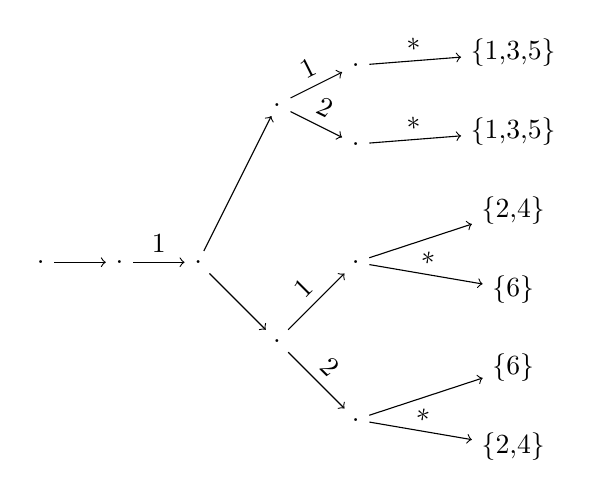
\begin{tikzpicture}[->,sloped,above]

	\node (root) at (0,2.5) {.};

	\node (h) at (1,2.5) {.};

	\node (h1) at (2,2.5) {.};

	\node (h1f) at (3,4.5) {.};
	\node (h1g) at (3,1.5) {.};

	\node (h1f1) at (4,5) {.};
	\node (h1f2) at (4,4) {.};
	\node (h1g1) at (4,2.5) {.};
	\node (h1g2) at (4,0.5) {.};

	\node (h1f1x) at (6,5) {\{1,3,5\}};
	\node (h1f2x) at (6,4) {\{1,3,5\}};
	\node (h1g1a) at (6,3) {\{2,4\}};
	\node (h1g1x) at (6,2) {\{6\}};
	\node (h1g2a) at (6,1) {\{6\}};
	\node (h1g2x) at (6,0) {\{2,4\}};

	\path (root) edge node {\( \mh \)} (h)
	(h) edge node {\( 1 \)} (h1)

	(h1)
	edge node {\( \mf \)} (h1f)
	edge node {\( \mg \)} (h1g)

	(h1f)
	edge node {\( 1 \)} (h1f1)
	edge node {\( 2 \)} (h1f2)

	(h1g)
	edge node {\( 1 \)} (h1g1)
	edge node {\( 2 \)} (h1g2)

	(h1f1)
	% edge node {\( \ma \)} (h1f1a)
	edge node {\( * \)} (h1f1x)

	(h1f2)
	%		edge node {\( \ma \)} (h1f2a)
	edge node {\( * \)} (h1f2x)


	(h1g1)
	edge node {\( \ma \)} (h1g1a)
	edge node {\( * \)} (h1g1x)

	(h1g2)
	edge node {\( \ma \)} (h1g2a)
	edge node {\( * \)} (h1g2x)
	;
	\end{tikzpicture}
\end{center}
\( \mh(\mg(y,x)) \mapsto \{ \mh.1.\mg.1.{*}, \mh.1.\mg.2.{*} \} \)
\end{example}

%+ PATH INDEXING/Retrieve
\begin{example}{Retrieve}
	\def\TRIEWIDTH{5cm}
	\def\TEXTWIDTH{\textwidth-\TRIEWIDTH-2em}

	\begin{minipage}{\TEXTWIDTH}
		\(
		\TI{t_1}\mh(\mf(x,y)),
		\TI{t_2}\mh(\mf({ x},{\ma})),
		\TI{t_3}\mh(\mf(\ma,\ma))
		 \)
		\begin{align*}
		\mh(\mf(z,\mb)) &\Rightarrow \{ \mh.1.\mf.1.{*}, \mh.1.\mf.2.\mb \}
		\\[0.7em]
		u : \mh(\mf({\colN z},{\colHi \mb}))
		& \mapsto
		{
			\{ t_1, {\colG t_2},
			{t_3} \}
		}
		{
			\cap \{t_1 \}
		}\\
%		{
			i : \mh(\mf(z, \mb)) &\mapsto \{ {\colG t_1,t_2,t_3 } \} \cap \{  \}
%		}
	\\
%		{
			g : \mh(\mf(z, \mb)) &\mapsto \{ t_1, {\colG t_2} \} \cap \{ t_1 \}
%		}
	\\
%		{
			v : \mh(\mf(z, \mb)) &\mapsto \{ {\colG t_1,t_2 }\} \cap \{  \}
%		}
	\\[0.7em]
%		{
			\colG v: \mh(\mf(z, z)) &\mapsto \{ {\colLo t_1},{\colG t_2} \} \cap \{ {\colLo t_1} \}
%		}
	\end{align*}
	\end{minipage}
	%
	\begin{minipage}{{\TRIEWIDTH}}
		\begin{tikzpicture}[->,dotted]
%		\input{PATHINDEXING/Index}
		\input{samples/pathindexingindex}

		\path[bend right, dashed, colN](root) edge (h);
		\node at (1.3,5) {\scriptsize\( (\mh,1.\mf.1.{*}) \)};
		\path[bend right, dashed, colN]	(h) edge (h1);
		\node at (1.0,4) {\scriptsize\( (1,\mf.1.{*}) \)};
		\path[bend right, dashed, colN]	(h1) edge (h1f);
		\node at (0.7,3) {\scriptsize\( (\mf,1.{*}) \)};
		\path[bend right, dashed, colN]	(h1f) edge (h1f1);
		\node at (0.4,2) {\scriptsize\( (1,{*}) \)};
		\path[bend right, dashed, colN]	(h1f1) edge (h1f1x)	;
		\node at (0.1,1) {\scriptsize\( ({*},\epsilon) \)};
		\path[bend right, dashed, colN]	(h1f1) edge (h1f1a);

		\path[bend left, dashed, colHi]	(root) edge (h)	;
		\node at (3.5,5) {\scriptsize\( (\mh,1.\mf.2.\mb) \)};
		\path[bend left, dashed, colHi]	(h) edge (h1)	;
		\node at (3.4,4) {\scriptsize\( (1,\mf.2.\mb) \)};
		\path[bend left, dashed, colHi]	(h1) edge (h1f)	;
		\node at (3.3,3) {\scriptsize\( (\mf,2.\mb) \)};
		\path[bend left, dashed, colHi]	(h1f) edge (h1f2)	;
		\node at (3.2,2) {\scriptsize\( (2,\mb) \)};
		\path[bend left, dashed, colHi]	(h1f2) edge (h1f2x)	;
		\node at (3.1,1) {\scriptsize\( (\mb,\epsilon) \)};
		\end{tikzpicture}
	\end{minipage}
\end{example}

%+ PATH INDEXING/Subterms
\begin{example}{Demodulation (Subterms)}

	\(
	\colG
	\TI{t_1}\mh(\mf(x,y)),
	\TI{t_2}\mh(\mf({ x},{\ma})),
	\TI{t_3}\mh(\mf(\ma,\ma)),
	\ldots,
%	\color{black}\mf(x,\ma) \foEQ x
	\color{black}\mf(x,\ma) \mEQ x
	 \)


	 \def\TRIEWIDTH{\textwidth/2-1em}% chktex 8
	 \def\TEXTWIDTH{\textwidth-\TRIEWIDTH-2em}
	\begin{minipage}{\TEXTWIDTH}
		\begin{tikzpicture}[->,dotted]
%		\input{PATHINDEXING/Index}
		\input{samples/pathindexingindex}

		\node (f) at (1.5,4) {.};
		\path[colN] (root) edge node {f} (f);

		\node (f1) at (0.5,4) {.};
		\path[colN] (f) edge node {1} (f1);

		\node (f1x) at (-0.5,4) {};
		\path[colN] (f1)	edge node {*} (f1x);

		\node[colN] (t1) at (-0.5,4.2) {\scriptsize\( t_1^1 \)};
		\node[colN] (t1) at (-0.5,3.8) {\scriptsize\(  t_2^1 \)};

		\node (f1a) at (-0.5,3) {};
		\path[colN] (f1) edge node {a} (f1a);

		\node[colN] (t3) at (-0.5,2.9) {\scriptsize\( t_3^1 \)};

		\node (f2) at (0.5,3) {.};
		\path[colN] (f) edge node {2}  (f2);

		\node (f2x) at (-0.5,2) {};
		\path[colN] (f2) edge node {*} (f2x);

		\node[colN] (t1) at (-0.5,1.9) {\scriptsize\( t_1^1 \)};

		\node (f2a) at (0.5,2) {};
		\path[colN] (f2) edge node {a} (f2a);

		\node[colN] (t2t3) at (0.5,1.9) {\scriptsize\( t_2^1,t_3^1 \)};

		\node (a) at (3.5,4) {};
		\path[colN] (root)  edge node {\( \ma \)} (a);
		\node[colN] (t2t3t3) at (3.5,3.9) {\scriptsize\( t_2^{12},t_3^{11,12} \)};

		\end{tikzpicture}
	\end{minipage}
	\hfill
	\begin{minipage}{{\TRIEWIDTH}}
		\def\pyL{-0.2}
		\def\pxL{0.05}
		\begin{tikzpicture}[->,dotted]
%		\input{PATHINDEXING/Index}
		\input{samples/pathindexingindex}

		\node[colN] (n-hsubs) at (5,4) {\( \mh \)};
		\path[dashdotted, above, pos=0.3,sloped,bend right=5,colN]  (n-hsubs) edge node {\scriptsize\( \ANGLES{\epsilon,\mh} \)} (h);

		\node[colN] (n-fsubs) at (5,3) {\( \mf \)};
		\path[dashdotted, above, pos=0.3,sloped, bend right=10,colN]  (n-fsubs) edge node {\scriptsize\( \ANGLES{1,\mf} \)} (h1f);

		\node[colN] (n-asubs) at (5,2) {\( \ma \)};
		\path[dashdotted, above, bend right, pos=0.3,sloped,colN]  (n-asubs) edge node {\scriptsize\( \ANGLES{11,\ma} \)} (h1f1a);
		\path[dashdotted, bend right, below, pos=0.3,sloped,colN]  (n-asubs) edge node {\scriptsize\( \ANGLES{12,\ma} \)} (h1f2a);

		\end{tikzpicture}
	\end{minipage}


\end{example}

%+ PATH INDEXING/SubtermTrees
\begin{example}{Subterm trees}
\begin{gather*}
\{
\TI{1}\mh(\mf(x,x)),
\TI{2}\mh(\mg(\ma,x)),
\TI{3}\mh(\mf(y,z))
\TI{4}\mh(\mg(\ma,y)),
\TI{5}\mh(\mf(y,x)),
\TI{6}\mh(\mg(y,a))
\}
\end{gather*}
%
\begin{center}
	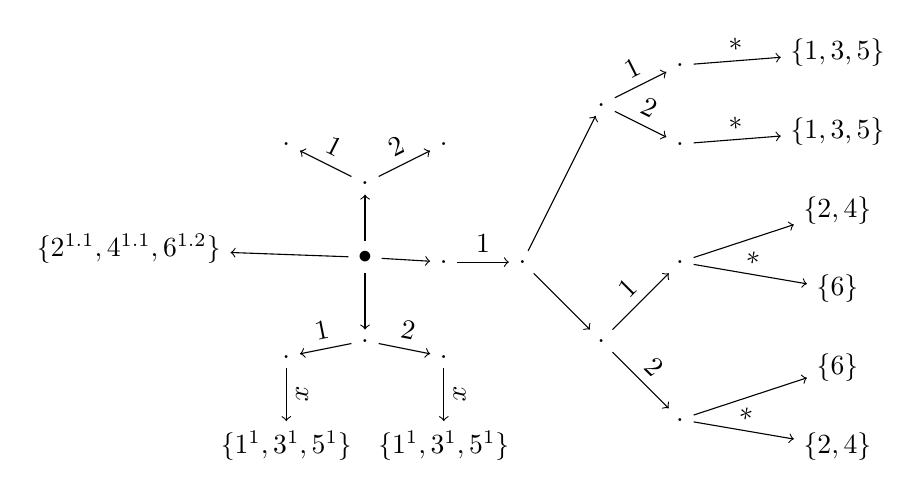
\begin{tikzpicture}[->,sloped,above]
	\node (root) at (0,2.5) {\( \bullet \)};
	%% right
	\node (h) at (1,2.5) {.};
	%
	\node (h1) at (2,2.5) {.};
	%
	\node (h1f) at (3,4.5) {.};
	\node (h1g) at (3,1.5) {.};
	%
	\node (h1f1) at (4,5) {.};
	\node (h1f2) at (4,4) {.};
	\node (h1g1) at (4,2.5) {.};
	\node (h1g2) at (4,0.5) {.};
	%
	\node (h1f1x) at (6,5) {\( \{1,3,5\} \)};
	\node (h1f2x) at (6,4) {\( \{1,3,5\} \)};
	\node (h1g1a) at (6,3) {\( \{2,4\} \)};
	\node (h1g1x) at (6,2) {\( \{6\} \)};
	\node (h1g2a) at (6,1) {\( \{6\} \)};
	\node (h1g2x) at (6,0) {\( \{2,4\} \)};
	%% down
	\node (f) at (0,1.5) {.};
	\node (f1) at (-1,1.3) {.};
	\node (f1x) at (-1,0) {\( \{1^{1},3^{1},5^{1}\} \)};
	\node (f2) at (1,1.3) {.};
	\node (f2x) at (1,0) {\( \{1^{1},3^{1},5^{1}\} \)};
	%% up
	\node (g) at (0,3.5) {.};
	\node (g1) at (-1,4) {.};
	\node (g2) at (1,4) {.};
	%% left
	\node (a) at (-3,2.5) {\( \{2^{1.1}, 4^{1.1}, 6^{1.2}\} \)};

	\path
	(root)
	edge node {\( \mh \)} (h)
	edge node {\( \mf \)} (f)
	edge node {\( \mg \)} (g)
	edge node {\( \ma \)} (a)

	(h) edge node {\( 1 \)} (h1)


	(h1)
	edge node {\( \mf \)} (h1f)
	edge node {\( \mg \)} (h1g)

	(h1f)
	edge node {\( 1 \)} (h1f1)
	edge node {\( 2 \)} (h1f2)

	(h1g)
	edge node {\( 1 \)} (h1g1)
	edge node {\( 2 \)} (h1g2)

	(h1f1)
	edge node {\( * \)} (h1f1x)

	(h1f2)
	edge node {\( * \)} (h1f2x)


	(h1g1)
	edge node {\( \ma \)} (h1g1a)
	edge node {\( * \)} (h1g1x)

	(h1g2)
	edge node {\( \ma \)} (h1g2a)
	edge node {\( * \)} (h1g2x)

	%
	(g) 	edge node {\( 1 \)} (g1)
	edge node {\( 2 \)} (g2)

	(f)	edge node {\( 1 \)} (f1)
	edge node {\( 2 \)} (f2)

	(f1)	edge node {\( x \)} (f1x)
	(f2)	edge node {\( x \)} (f2x)
	;


	\path (root)



	;

	\end{tikzpicture}
\end{center}
\end{example}





\subsection{Substitution Tree}
%% SUBSTITUTION TREES

%+ SUBSTITUTION TREES/Build+Index
\begin{example}{Substitution tree build}

	\(
	\TI{t_1}\mh(\mf(x,y)),
	\TI{t_2}\mh(\mf(x,\mh(\ma))),
	\TI{t_3}\mh(\mf(\mh(\ma),\ma)),
	\TI{t_4}\mh(\mf(\ma,\ma))
	 \)

	\begin{tikzpicture}[->]
%	\input{SUBSTITUTION TREES/Index}
	\ORIGIN


\node (root) at (0,0) {.};
\node (h) at (0,-1) {$*_0 \mapsto \mh(*_1)$};
\path (root) edge (h);

\node (f) at (0,-2) {$*_1 \mapsto \mf(*_2,*_3)$};
\path (h) edge (f);

\node (x2x) at (-2,-3) {$*_2 \mapsto x$} ;
\path (f) edge (x2x);

\node (x3y) at (-3,-4) {$*_3 \mapsto y$};
\path (x2x) edge (x3y);
\node (t1) at (-3,-4.4) {$t_1$};

\node (x3ha) at (-1,-4) {$*_3 \mapsto \mh(\ma)$};
\path (x2x) edge (x3ha);
\node (t2) at (-1,-4.4) {$t_2$};

\node (x3a)at (2,-3) {$*_3\mapsto\ma$};
\path (f) edge (x3a);

\node (x2ha) at (1,-4) {$*_2\mapsto\mh(\ma)$};
\path (x3a) edge (x2ha);
\node (t3) at (1,-4.4) {$t_3$};

\node (x2a) at (3,-4) {$*_2\mapsto\ma$};
\path (x3a) edge (x2a);
\node (t4) at (3,-4.4) {$t_4$};

	\end{tikzpicture}
\end{example}

%+ SUBSTITUTION TREES/Retrieve+Index
\begin{example}{Substitution tree retrieve}

	\(
	\TI{t_1}\mh(\mf(x,y)),
	\TI{t_2}\mh(\mf(x,\mh(\ma))),
	\TI{t_3}\mh(\mf(\mh(\ma),\ma)),
	\TI{t_4}\mh(\mf(\ma,\ma))
	 \)

	\begin{tikzpicture}[->]
%	\input{SUBSTITUTION TREES/Index}
	\ORIGIN


\node (root) at (0,0) {.};
\node (h) at (0,-1) {$*_0 \mapsto \mh(*_1)$};
\path (root) edge (h);

\node (f) at (0,-2) {$*_1 \mapsto \mf(*_2,*_3)$};
\path (h) edge (f);

\node (x2x) at (-2,-3) {$*_2 \mapsto x$} ;
\path (f) edge (x2x);

\node (x3y) at (-3,-4) {$*_3 \mapsto y$};
\path (x2x) edge (x3y);
\node (t1) at (-3,-4.4) {$t_1$};

\node (x3ha) at (-1,-4) {$*_3 \mapsto \mh(\ma)$};
\path (x2x) edge (x3ha);
\node (t2) at (-1,-4.4) {$t_2$};

\node (x3a)at (2,-3) {$*_3\mapsto\ma$};
\path (f) edge (x3a);

\node (x2ha) at (1,-4) {$*_2\mapsto\mh(\ma)$};
\path (x3a) edge (x2ha);
\node (t3) at (1,-4.4) {$t_3$};

\node (x2a) at (3,-4) {$*_2\mapsto\ma$};
\path (x3a) edge (x2a);
\node (t4) at (3,-4.4) {$t_4$};
	\end{tikzpicture}
\end{example}

%% DISCRIMINATION TREE
\subsection{Discrimination Tree}

%\ORIGIN

\node (root) at (1,0) {.};
\node (h) at (0,-1) {.};
\path (root) edge node {\( \mh \)} (h);
\node (hf) at (-1,-2) {.};
\path (h) edge node {\( \mf \)} (hf);
\node (hfx) at (-2,-3) {.};
\path (hf) edge node {\( * \)} (hfx);
\node (n-hfxx) at (-3,-4) {.};
\path (hfx) edge node {\( * \)} (n-hfxx);
\node (1) at (-3,-4.2) {\scriptsize \( t_1 \)};

\node (n-hfxh) at (-2,-4) {.};
\path (hfx) edge node {\( \mh \)} (n-hfxh);
\node (n-hfxha) at (-2,-5) {.};
\path (n-hfxh) edge node {\( \ma \)} (n-hfxha);
\node (2) at (-2,-5.2) {\scriptsize \( t_2 \)};

\node (hfh) at (-1,-3) {.};
\path (hf) edge node {\( \mh \)} (hfh);
\node (n-hfha) at (-1,-4) {.};
\path (hfh) edge node {\( \ma \)} (n-hfha);
\path[dashdotted,bend left=45,gray] (hf) edge (n-hfha);
\node (n-hfhaa) at (-1,-5) {.};
\path (n-hfha) edge node {\( \ma \)} (n-hfhaa);
\node (3) at (-1,-5.2) {\scriptsize \( t_3 \)};
%\input{samples/discriminationtreeterms}
%% DISCRIMINATION TREE/Build+Terms+Index
\begin{example}{Build}

	\def\TRIEWIDTH{4.4cm}
	\def\TEXTWIDTH{\textwidth-\TRIEWIDTH-2em}
	\begin{minipage}{\TEXTWIDTH}
%		$
\TI{\ell_1}\mP(\mf(x,y)), 
\TI{\ell_2}\mP(\mf(x,\mh(\ma))),
\TI{\ell_3}\mP(\mf(\mh(\ma),\ma))
$
		\input{samples/discriminationtreeterms}
		\begin{align*}
		t_1 &\Rightarrow \mh.\mf.{*}.{*}\\
		t_2 &\Rightarrow \mh.\mf.{*}.\mh.\ma \\
		t_3 &\Rightarrow \mh.\mf.\mh.\ma.\ma
		\end{align*}
	\end{minipage}
	\begin{minipage}{\TRIEWIDTH}
		\def\pyL{-0.3}
		\def\pxL{-0.0}
		\begin{tikzpicture}[->,dotted]
%		\input{DISCRIMINATION TREE/Index}
		\ORIGIN

\node (root) at (1,0) {.};
\node (h) at (0,-1) {.};
\path (root) edge node {\( \mh \)} (h);
\node (hf) at (-1,-2) {.};
\path (h) edge node {\( \mf \)} (hf);
\node (hfx) at (-2,-3) {.};
\path (hf) edge node {\( * \)} (hfx);
\node (n-hfxx) at (-3,-4) {.};
\path (hfx) edge node {\( * \)} (n-hfxx);
\node (1) at (-3,-4.2) {\scriptsize \( t_1 \)};

\node (n-hfxh) at (-2,-4) {.};
\path (hfx) edge node {\( \mh \)} (n-hfxh);
\node (n-hfxha) at (-2,-5) {.};
\path (n-hfxh) edge node {\( \ma \)} (n-hfxha);
\node (2) at (-2,-5.2) {\scriptsize \( t_2 \)};

\node (hfh) at (-1,-3) {.};
\path (hf) edge node {\( \mh \)} (hfh);
\node (n-hfha) at (-1,-4) {.};
\path (hfh) edge node {\( \ma \)} (n-hfha);
\path[dashdotted,bend left=45,gray] (hf) edge (n-hfha);
\node (n-hfhaa) at (-1,-5) {.};
\path (n-hfha) edge node {\( \ma \)} (n-hfhaa);
\node (3) at (-1,-5.2) {\scriptsize \( t_3 \)};
		\node (lu) at (-3,-5.5) {} ;
		\end{tikzpicture}
	\end{minipage}
	%
\end{example}



%% DISCRIMINATION TREE/Index
%% DISCRIMINATION TREE/IndexEdges

%+ DISCRIMINATION TREE/Retrieve+Terms+Index
\begin{example}{Retrieve}

	\def\TRIEWIDTH{4.4cm}
	\def\TEXTWIDTH{\textwidth-\TRIEWIDTH-2em}
	\begin{minipage}{\TEXTWIDTH}
%		$
\TI{\ell_1}\mP(\mf(x,y)), 
\TI{\ell_2}\mP(\mf(x,\mh(\ma))),
\TI{\ell_3}\mP(\mf(\mh(\ma),\ma))
$
		\input{samples/discriminationtreeterms}
		\begin{align*}
		\mh(\mf(x',\ma))&\Rightarrow \mh.\mf.{*}.\ma
		\\[0.7em]
		u: \mh(\mf(x',\ma))&\mapsto \{
		{t_1,}
		{t_3}
		\}
		\\
					i:\mh(\mf(x',\ma))&\mapsto \{t_3\}  \\
					g:\mh(\mf(x',\ma))&\mapsto \{t_1\} \\
					v:\mh(\mf(x',\ma))&\mapsto \{  \} \\
		\end{align*}
	\end{minipage}
%
	\begin{minipage}{\TRIEWIDTH}
		\begin{tikzpicture}[->,dotted]
%		\input{DISCRIMINATION TREE/Index}
		\ORIGIN

\node (root) at (1,0) {.};
\node (h) at (0,-1) {.};
\path (root) edge node {\( \mh \)} (h);
\node (hf) at (-1,-2) {.};
\path (h) edge node {\( \mf \)} (hf);
\node (hfx) at (-2,-3) {.};
\path (hf) edge node {\( * \)} (hfx);
\node (n-hfxx) at (-3,-4) {.};
\path (hfx) edge node {\( * \)} (n-hfxx);
\node (1) at (-3,-4.2) {\scriptsize \( t_1 \)};

\node (n-hfxh) at (-2,-4) {.};
\path (hfx) edge node {\( \mh \)} (n-hfxh);
\node (n-hfxha) at (-2,-5) {.};
\path (n-hfxh) edge node {\( \ma \)} (n-hfxha);
\node (2) at (-2,-5.2) {\scriptsize \( t_2 \)};

\node (hfh) at (-1,-3) {.};
\path (hf) edge node {\( \mh \)} (hfh);
\node (n-hfha) at (-1,-4) {.};
\path (hfh) edge node {\( \ma \)} (n-hfha);
\path[dashdotted,bend left=45,gray] (hf) edge (n-hfha);
\node (n-hfhaa) at (-1,-5) {.};
\path (n-hfha) edge node {\( \ma \)} (n-hfhaa);
\node (3) at (-1,-5.2) {\scriptsize \( t_3 \)};
		\path[bend right, dashed, colN] (root) edge  (h);
		\path[bend right, dashed, colN] (h) edge  (hf);
		\path[bend right, dashed, colN] (hf) edge (hfx);
		\path[bend right, dashed, colN] (hfx) edge  (n-hfxx);
		\path[bend right, dashed, colN] (hf) edge  (n-hfha);
		\path[bend right, dashed, colN] (n-hfha) edge (n-hfhaa);

		\node (lu) at (-3,-5.5) {} ;
		\end{tikzpicture}
	\end{minipage}
	%
\end{example}

%% DISCRIMINATION TREE/Subterms+Terms+Index
\begin{example}{Subterms}
	\def\TRIEWIDTH{\textwidth/2-1em}% chktex 8
%%	$
\TI{\ell_1}\mP(\mf(x,y)), 
\TI{\ell_2}\mP(\mf(x,\mh(\ma))),
\TI{\ell_3}\mP(\mf(\mh(\ma),\ma))
$
	\input{samples/discriminationtreeterms}
%	\vspace{1em}

	\begin{minipage}{\TRIEWIDTH}
		\begin{tikzpicture}[->, dotted]
%		\input{DISCRIMINATION TREE/Index}
		\ORIGIN

\node (root) at (1,0) {.};
\node (h) at (0,-1) {.};
\path (root) edge node {\( \mh \)} (h);
\node (hf) at (-1,-2) {.};
\path (h) edge node {\( \mf \)} (hf);
\node (hfx) at (-2,-3) {.};
\path (hf) edge node {\( * \)} (hfx);
\node (n-hfxx) at (-3,-4) {.};
\path (hfx) edge node {\( * \)} (n-hfxx);
\node (1) at (-3,-4.2) {\scriptsize \( t_1 \)};

\node (n-hfxh) at (-2,-4) {.};
\path (hfx) edge node {\( \mh \)} (n-hfxh);
\node (n-hfxha) at (-2,-5) {.};
\path (n-hfxh) edge node {\( \ma \)} (n-hfxha);
\node (2) at (-2,-5.2) {\scriptsize \( t_2 \)};

\node (hfh) at (-1,-3) {.};
\path (hf) edge node {\( \mh \)} (hfh);
\node (n-hfha) at (-1,-4) {.};
\path (hfh) edge node {\( \ma \)} (n-hfha);
\path[dashdotted,bend left=45,gray] (hf) edge (n-hfha);
\node (n-hfhaa) at (-1,-5) {.};
\path (n-hfha) edge node {\( \ma \)} (n-hfhaa);
\node (3) at (-1,-5.2) {\scriptsize \( t_3 \)};
		\node (ha) at (1,-2) {.} ;
		\path[dashdotted,colN] (h) edge node {\( \ma \)} (ha);
		\node (tha)  at (1,-2.2) {\scriptsize\( t_2^{{\colN 12}}, t_3^{{\colN 111}} \)} ;
		{(lu) at (-3.5,-5.5) {+}}

		\end{tikzpicture}
	\end{minipage}
%	\hfill{
		\begin{minipage}{\TRIEWIDTH}
			\begin{tikzpicture}[->,dotted]
%
%%			\input{DISCRIMINATION TREE/Index}
			\ORIGIN

\node (root) at (1,0) {.};
\node (h) at (0,-1) {.};
\path (root) edge node {\( \mh \)} (h);
\node (hf) at (-1,-2) {.};
\path (h) edge node {\( \mf \)} (hf);
\node (hfx) at (-2,-3) {.};
\path (hf) edge node {\( * \)} (hfx);
\node (n-hfxx) at (-3,-4) {.};
\path (hfx) edge node {\( * \)} (n-hfxx);
\node (1) at (-3,-4.2) {\scriptsize \( t_1 \)};

\node (n-hfxh) at (-2,-4) {.};
\path (hfx) edge node {\( \mh \)} (n-hfxh);
\node (n-hfxha) at (-2,-5) {.};
\path (n-hfxh) edge node {\( \ma \)} (n-hfxha);
\node (2) at (-2,-5.2) {\scriptsize \( t_2 \)};

\node (hfh) at (-1,-3) {.};
\path (hf) edge node {\( \mh \)} (hfh);
\node (n-hfha) at (-1,-4) {.};
\path (hfh) edge node {\( \ma \)} (n-hfha);
\path[dashdotted,bend left=45,gray] (hf) edge (n-hfha);
\node (n-hfhaa) at (-1,-5) {.};
\path (n-hfha) edge node {\( \ma \)} (n-hfhaa);
\node (3) at (-1,-5.2) {\scriptsize \( t_3 \)};
			\node (n-hsubs) at (1,-4.5) {};
			\path[dashdotted, colN, sloped,above] (n-hsubs)
			edge[pos=0.4] node[sloped]
			{\scriptsize\( \ANGLES{\epsilon,\mh} \)}  (h);
			\path[dashdotted, colN,sloped, above] (n-hsubs)
			edge[bend left=0,pos=0.4,sloped]
			node
			{\scriptsize\( \ANGLES{11,\mh} \)}
			(hfh);
%
			\path[dashdotted, colN] (n-hsubs)
			edge[bend left=0,pos=0.2,sloped]
			node[below] {\scriptsize \( \ANGLES{12,\mh} \)}
			(n-hfxh);
%
			\node (lu) at (-3.5,-5.5) {} ;
			\end{tikzpicture}
	\end{minipage}
%	%
\end{example}










